\chapter{Bedienungsanleitung der Anwendung}
\label{Bedienungsanleitung}
Der Programmentwurf besitzt eine mithilfe der Angular-Technologie entwickelten Benutzeroberfläche, deren Anwendung im Folgenden erläutert wird.

\section{Aufrufen der Anwendung}
Die Angular-Anwendung lässt sich mittels des Befehls \code{npm start} im entsprechenden Oberverzeichnis starten.
Nach der Initialisierung ist die Anwendung entsprechend Abbildung \ref{fig:gui-initial-screen} über die Adresse \code{http://localhost:4200} erreichbar.

\begin{figure}[H]
	\centering
	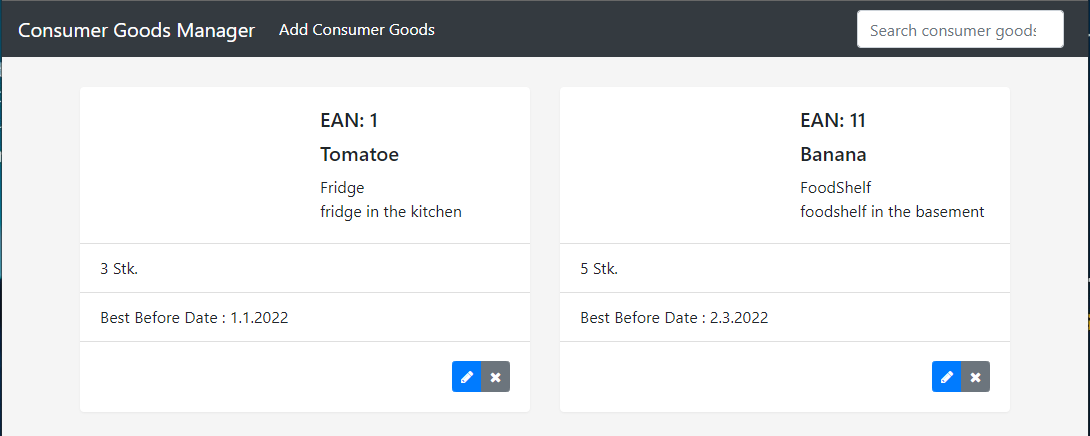
\includegraphics[width=1.0\textwidth]{Bilder/gui/gui-initial-screen.PNG}
	\caption[]{}
	\label{fig:gui-initial-screen}
\end{figure}

Auf der initialen Darstellung werden bereits verwaltete Konsumgüter dargestellt.
Über das Eingabefeld an der rechten oberen Seite können Konsumgüter entsprechend ihrer Attribute gesucht werden.

\begin{figure}[H]
	\centering
	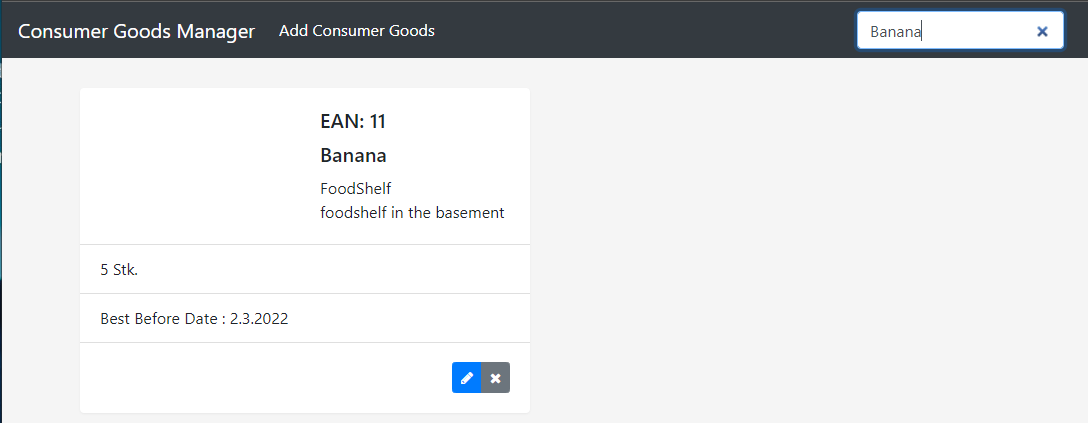
\includegraphics[width=1.0\textwidth]{Bilder/gui/gui-search.PNG}
	\caption[]{}
	\label{fig:gui-search}
\end{figure}

\section{Konsumgut anlegen}
\label{konsumgut-anlegen}
Das Anlegen eines Konsumguts ist über den Button \textit{Add Consumer Goods} möglich.
Darauf öffnet sich ein Fenster wie in Abbildung \ref{fig:gui-add-consumer} zur Eingabe der Daten des neuanzulegenden Konsumguts.
Nach Eingabe kann das Konsumgut über den Button \textit{Add Consumer Goods} angelegt werden.

\begin{figure}[H]
	\centering
	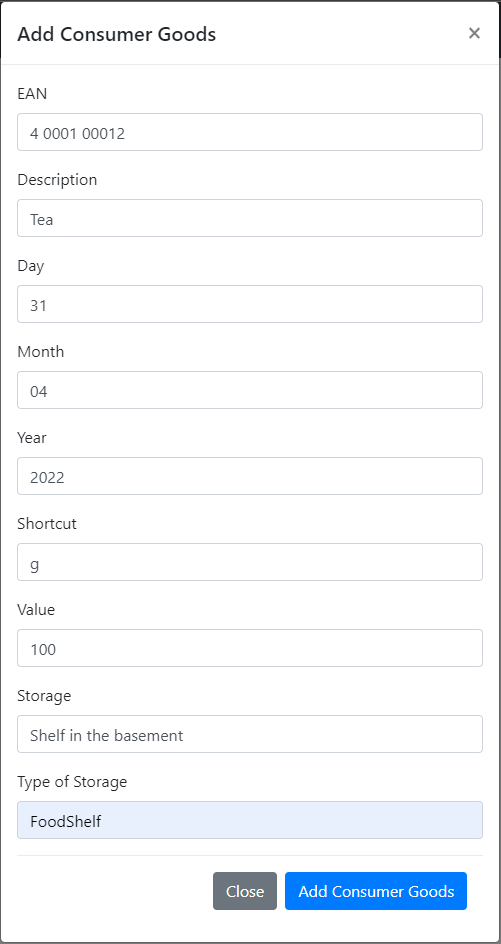
\includegraphics[width=0.3\textwidth]{Bilder/gui/add-consumer-goods.PNG}
	\caption[.]{}
	\label{fig:gui-add-consumer}
\end{figure}

Nachdem das Konsumgut angelegt ist, wird es ebenfalls auf der Oberfläche entsprechend Abbildung \ref{fig:gui-created-item} dargestellt.

\begin{figure}[H]
	\centering
	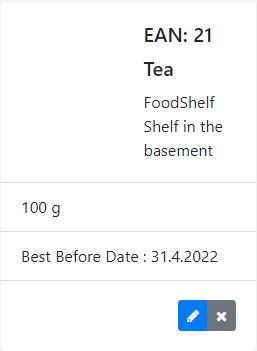
\includegraphics[width=0.3\textwidth]{Bilder/gui/gui-created-item.PNG}
	\caption[.]{.}
	\label{fig:gui-created-item}
\end{figure}

Über den blauen Button können die Attribute des Konsumguts geändert werden.
Das Vorgehen wird in Abschnitt \ref{konsumgut-aendern} beschrieben.
Über den grauen Button kann das Konsumgut gelöscht werden.
Das Vorgehen wird in Abschnitt \ref{konsumgut-loeschen} beschrieben.

\section{Daten eines Konsumsgut ändern}
\label{konsumgut-aendern}
Zum Ändern von Attributen eines Konsumguts muss der blaue Button des gewünschten Konsumguts ausgewählt werden.
Daraufhin öffnet sich eine Eingabemaske wie in Abbildung \ref{fig:gui-edit} gezeigt, in der die aktuellen Werte der Attribute enthalten sind.
Die Werte können entsprechend angepasst und durch Auswahl des Buttons \textit{Save changes} bestätigt werden.
\begin{figure}[H]
	\centering
	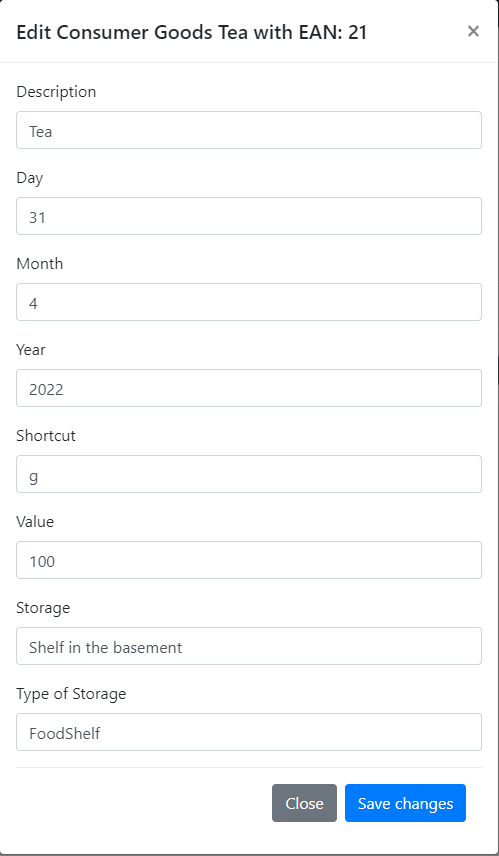
\includegraphics[width=0.3\textwidth]{Bilder/gui/gui-edit-consumer-goods.PNG}
	\caption[.]{.}
	\label{fig:gui-edit}
\end{figure}

\section{Konsumgut löschen}
\label{konsumgut-loeschen}
Das Löschen des Konsumguts erfolgt über den grauen Button.
Bei Auswahl öffnet sich ein Dialogfenster entsprechend Abbildung \ref{fig:gui-delete-item}, dass den Nutzer noch einmal auffordert, den Löschvorgang zu bestätigen, um ein unbeabsichtigtes Löschen zu vermeiden.

\begin{figure}[H]
	\centering
	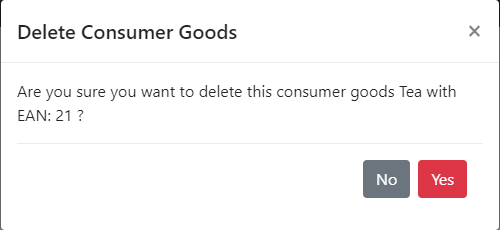
\includegraphics[width=0.7\textwidth]{Bilder/gui/gui-delete-consumer-goods.PNG}
	\caption[.]{.}
	\label{fig:gui-delete-item}
\end{figure}
